\documentclass{standalone}

\usepackage{tikz}
\usepackage{bm}
\usepackage{amsmath}
\usetikzlibrary{calc, tikzmark, shapes, shapes.arrows, arrows, positioning}
\newcommand{\mat}[1]{\boldsymbol{\rm{#1}}}
\newcommand{\T}{\mat{T}}
\renewcommand{\vec}[1]{\boldsymbol{#1}}
\newcommand{\x}{\boldsymbol{\mathrm{x}}}
\newcommand{\pderiv}[2]{\frac{\partial #1}{\partial #2}}

\begin{document}
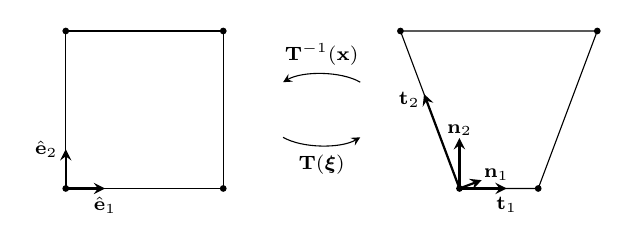
\begin{tikzpicture}
	\scriptsize
	\begin{scope}[xshift=0cm, scale=1]
		\draw (-1,-1) -- (1,-1) -- (1,1) -- (-1,1) -- (-1,-1); 
		\filldraw[black] (-1,-1) circle[radius=1pt]; 
		\filldraw[black] (1,-1) circle[radius=1pt]; 
		\filldraw[black] (1,1) circle[radius=1pt]; 
		\filldraw[black] (-1,1) circle[radius=1pt]; 
		\draw[>=stealth, ->, thick] (-1,-1) -- (-.5,-1) node[below] {$\hat{\mat{e}}_1$}; 
		\draw[>=stealth, ->, thick] (-1,-1) -- (-1,-.5) node[left] {$\hat{\mat{e}}_2$}; 
	\end{scope}
	\begin{scope}[xshift=2.25cm, yshift=0cm]
		\draw[->, >=stealth, shorten >= 3mm, shorten <= 3mm] (-.75,-.2) to [bend right=30] (.75,-.2); 
		\node at (0,-.7) {$\T(\vec{\xi})$}; 
		\draw[->, >=stealth, shorten >= 3mm, shorten <= 3mm] (.75,.2) to [bend right=30] (-.75,.2); 
		\node at (0,.7) {$\T^{-1}(\x)$}; 
	\end{scope}
	\begin{scope}[xshift=4.5cm, scale=1]
		\draw (-.5,-1) -- (.5,-1) -- (1.25,1) -- (-1.25,1) -- (-.5,-1); 
		\filldraw[black] (-.5,-1) circle[radius=1pt]; 
		\filldraw[black] (.5,-1) circle[radius=1pt]; 
		\filldraw[black] (1.25,1) circle[radius=1pt]; 
		\filldraw[black] (-1.25,1) circle[radius=1pt]; 
		\draw[>=stealth, ->, thick] (-.5,-1) -- +(0:.6cm) node[below] {$\mat{t}_1$}; 
		\draw[>=stealth, ->, thick] (-.5,-1) -- +(20.556045219583464:.3cm) node[shift={(20.556045219583464:.2cm)}] {$\mat{n}_1$};
		\draw[>=stealth, ->, thick] (-.5,-1) -- +(110.55604521958347:.3*1.068*4cm) node[shift={(110.55604521958347+90:.2cm)}] {$\mat{t}_2$}; 
		\draw[>=stealth, ->, thick] (-.5,-1) -- +(90:.3*1.068*2cm) node[shift={(90:.1cm)}] {$\mat{n}_2$}; 

		% \draw[>=stealth, ->, thick] (1.25,1) -- +(0:.5cm) node[shift={(0:.15cm)}] {$\vec{t}_1$}; 
		% \draw[>=stealth, ->, thick] (1.25,1) -- +(60.5397:.5cm) node[shift={(60.5397:.1cm)}] {$\vec{t}_2$};  
		% \draw[>=stealth, ->, thick] (1.25,1) -- +(-22.5531:.5cm) node[shift={(-22.5531:.2cm)}] {$\vec{n}_1$};
		% \draw[>=stealth, ->, thick] (1.25,1) -- +(90:.5cm) node[shift={(90:.1cm)}] {$\vec{n}_2$}; 

		% \draw[>=stealth, ->, thick] (7/8,0) -- +(0:.5cm) node[shift={(0:.15cm)}] {$\vec{t}_1$}; 
		% \draw[>=stealth, ->, thick] (7/8,0) -- +(67.4469:.5cm) node[shift={(67.4469:.1cm)}] {$\vec{t}_2$};  
		% \draw[>=stealth, ->, thick] (7/8,0) -- +(-22.5531:.5cm) node[shift={(-22.5531:.2cm)}] {$\vec{n}_1$};
		% \draw[>=stealth, ->, thick] (7/8,0) -- +(90:.5cm) node[shift={(90:.1cm)}] {$\vec{n}_2$};
	\end{scope}
\end{tikzpicture}
\end{document}